\documentclass[/home/jesse/Analysis/FemtoAnalysis/AnalysisNotes/AnalysisNoteJBuxton.tex]{subfiles}


\begin{document}

\subsubsection{Discussion of \mt-Scaling}
\label{ResultsLamK_DiscussionOfmTScaling}

Discuss why \mt scaling is not appropriate for non-identical femtoscopy studies.


\begin{figure}[h]
  \centering
  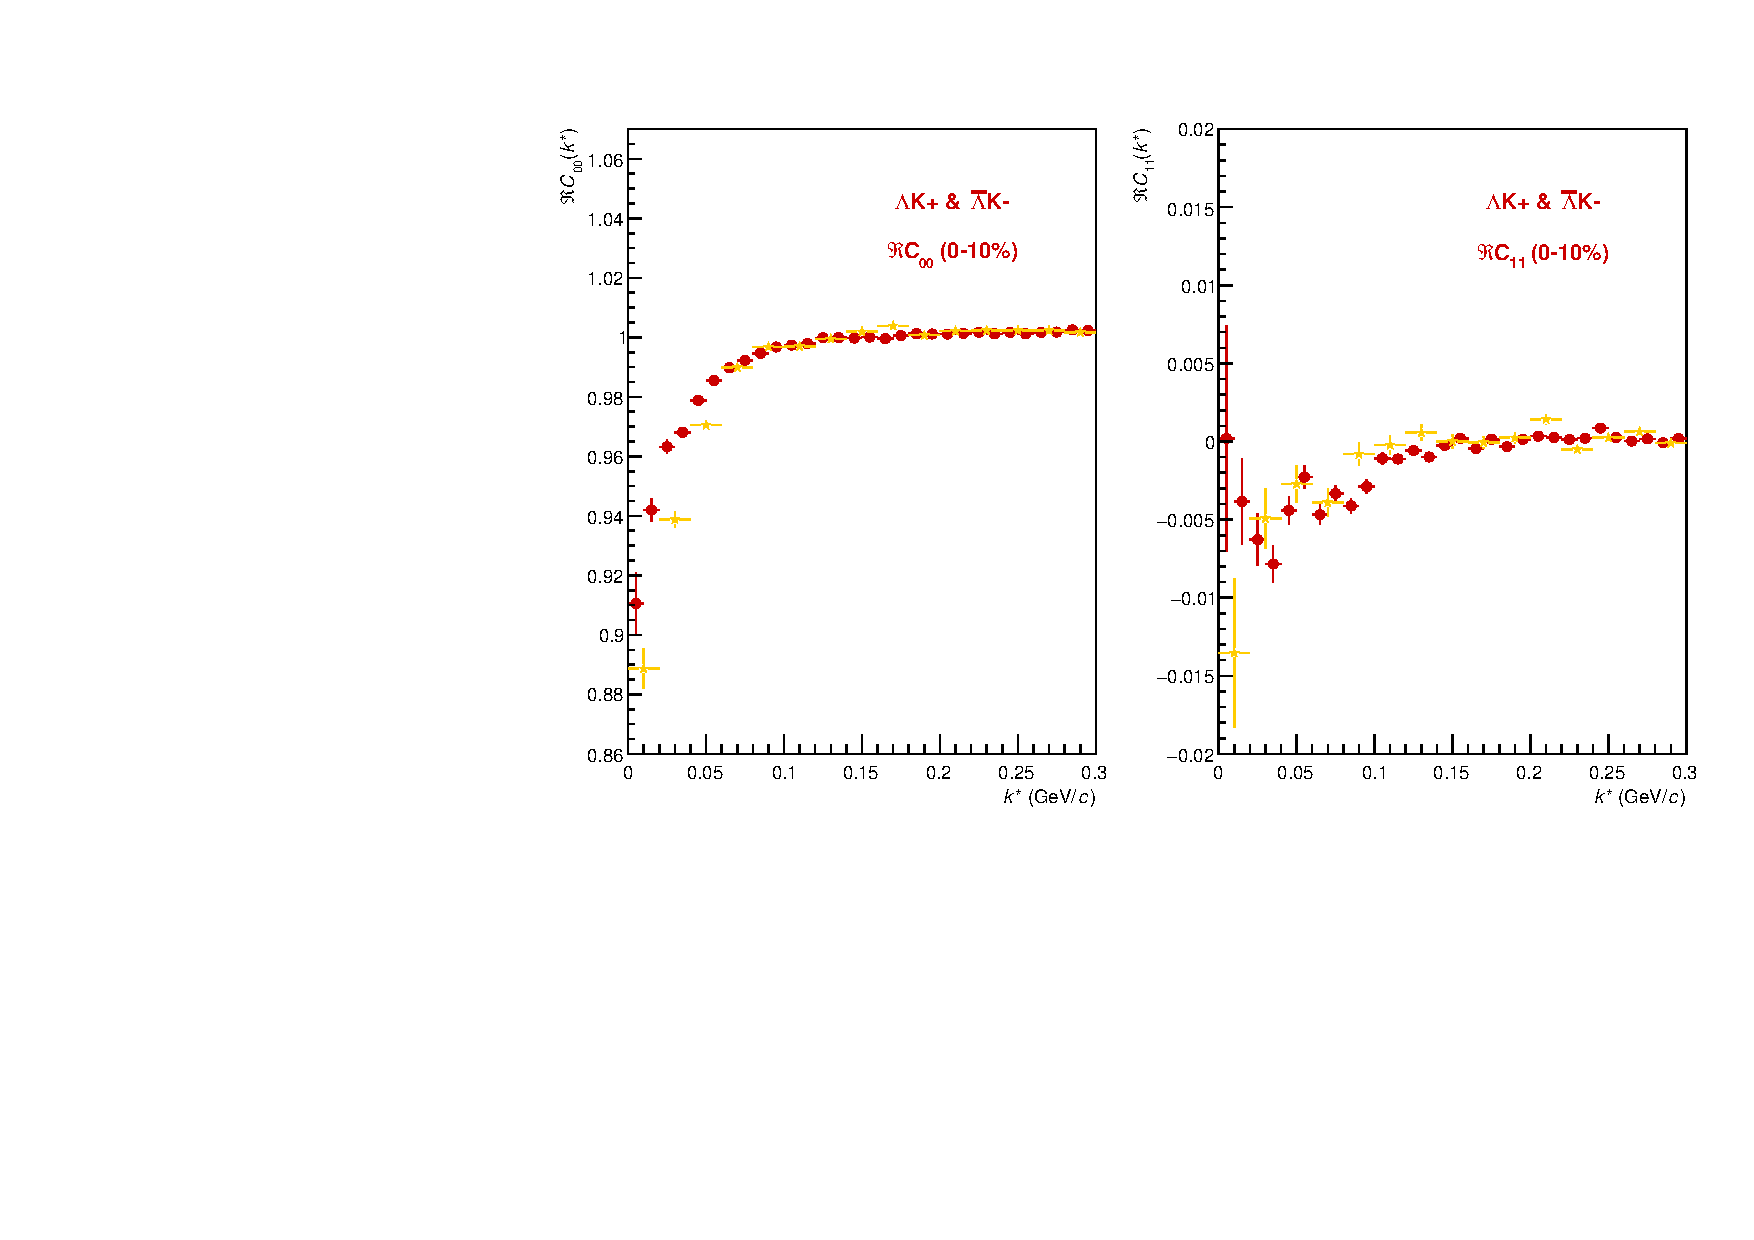
\includegraphics[width=\textwidth]{\ResultsDirBase Results_cLamcKch_20181205/SphericalHarmonics/LamKchP/CanCfYlmReC00C11_LamKchPALamKchM_0010.pdf}
  \caption[Short Caption]{Long Caption}
  \label{fig:LamKchP_ReC00C11_0010}
\end{figure}





\begin{figure}[h!]
  \centering
  %%----start of first subfigure---  
  \subfloat[Caption 1]{
    \label{fig:LamKchP_StdThermSources_Spatial}
    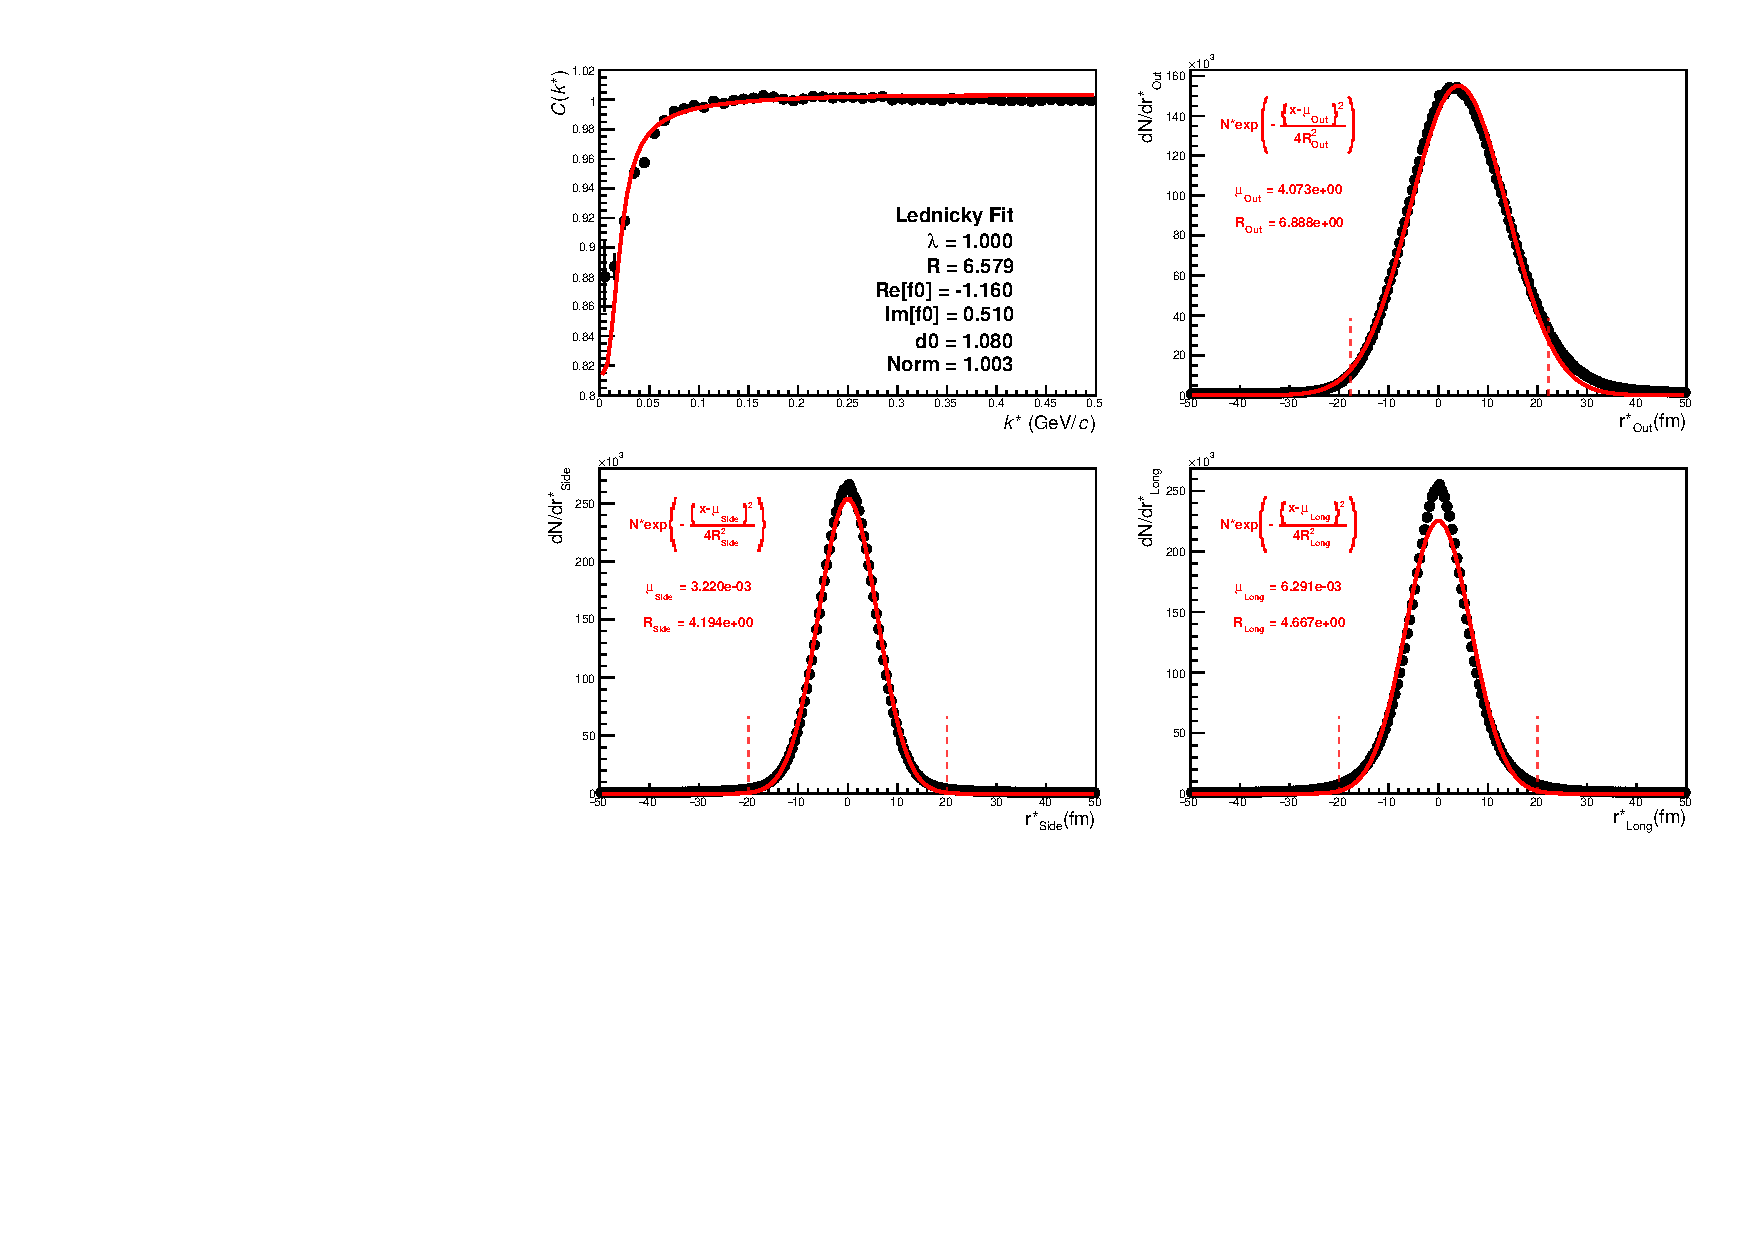
\includegraphics[width=\linewidth]{/home/jesse/Analysis/FemtoAnalysis/AnalysisNotes/7_ResultsAndDiscussion/7.1_ResultsLamK/7.1.5_ResultsLamK_DiscussionOfmTScaling/ThermPlots/LamKchP/CanCfwSource_Full_LamKchP_3dHistPairSource3d_oslLamKchP_FromFileCorrelationFunctions_wOtherPairs.pdf}} \\
  %%----start of second subfigure---
  \subfloat[Caption 2]{
    \label{fig:LamKchP_StdThermSources_Temporal}
    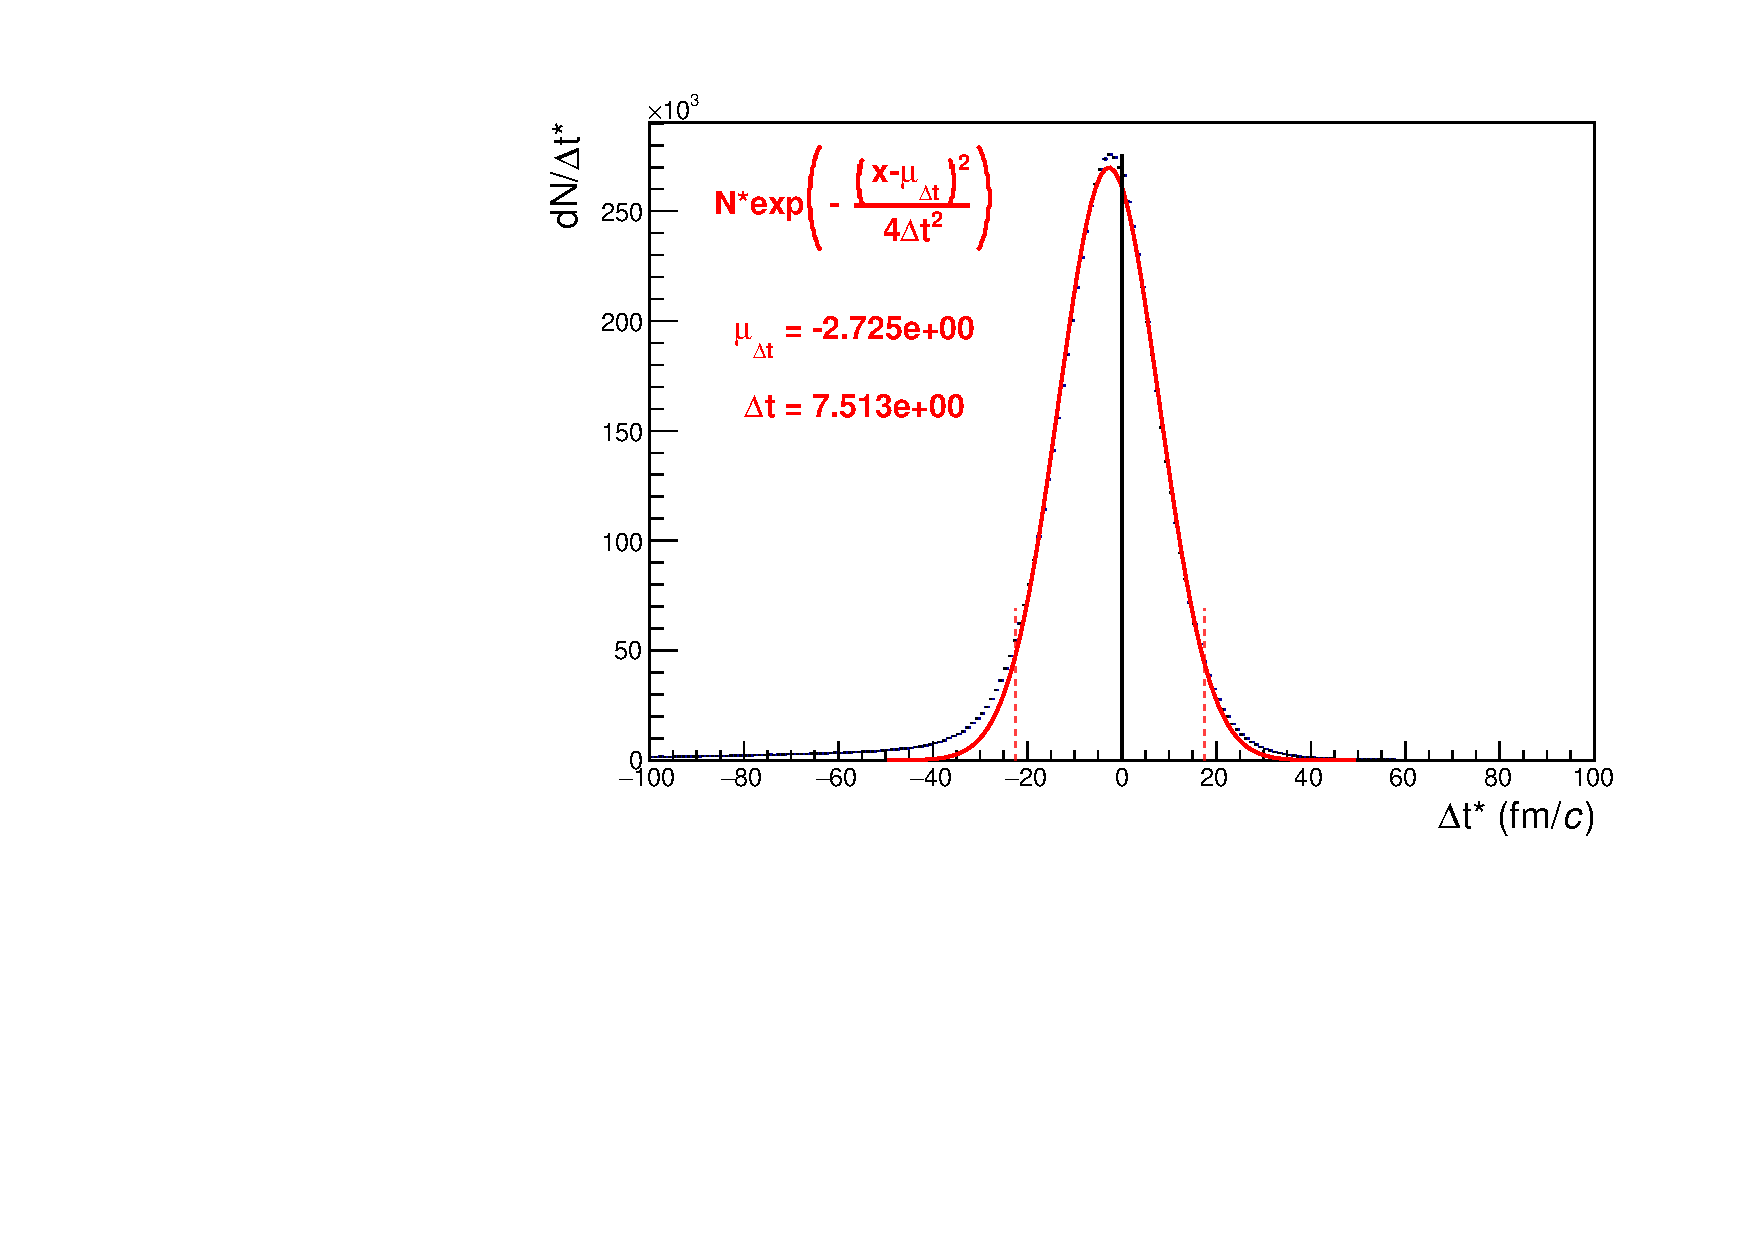
\includegraphics[width=0.60\linewidth]{/home/jesse/Analysis/FemtoAnalysis/AnalysisNotes/7_ResultsAndDiscussion/7.1_ResultsLamK/7.1.5_ResultsLamK_DiscussionOfmTScaling/ThermPlots/LamKchP/CanDeltaT_Full_LamKchP_FromFileCorrelationFunctions_wOtherPairs_BuildCfYlm.pdf}}  
  %%----overall caption----
  \caption[Short Overall]{Long Overall}
  \label{fig:LamKchP_StdThermSources}
\end{figure}














\begin{figure}[h]
  \centering
  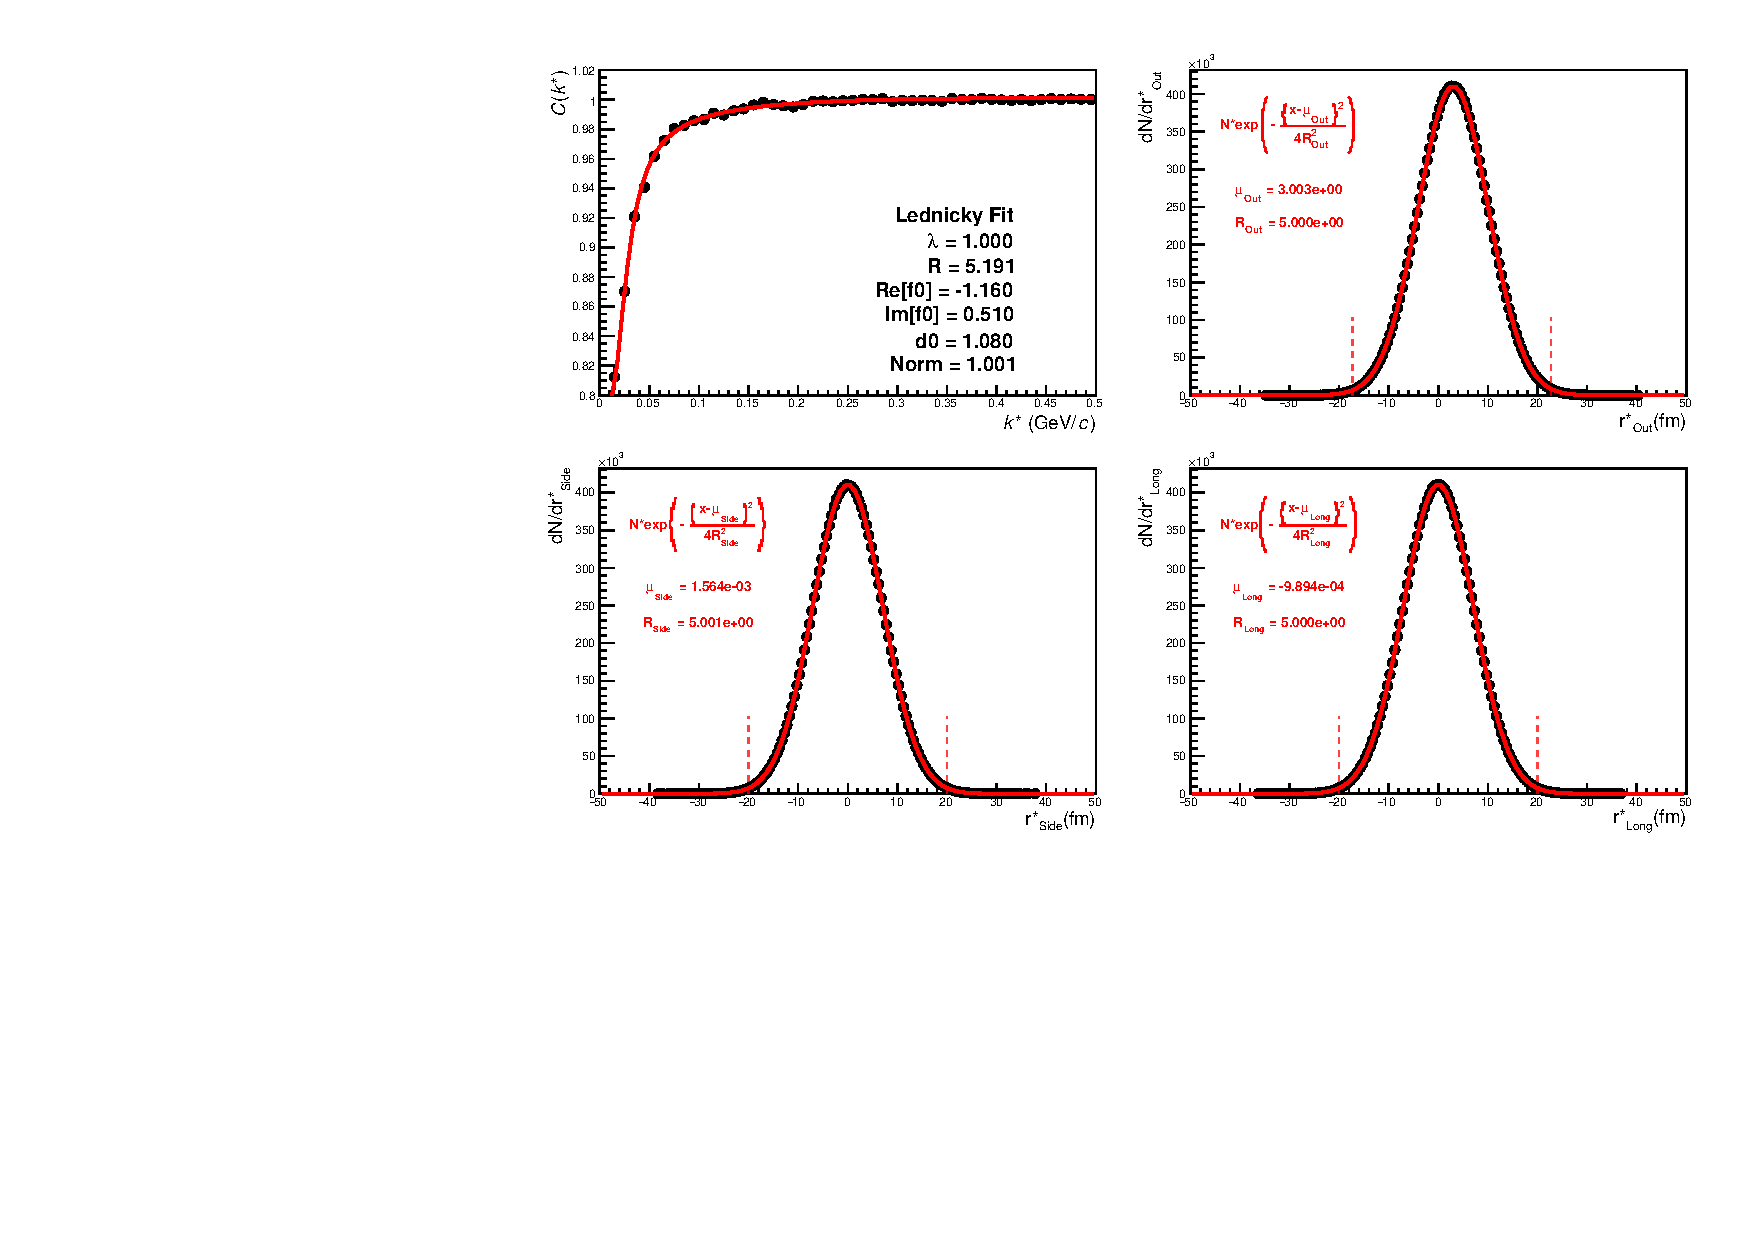
\includegraphics[width=\textwidth]{/home/jesse/Analysis/FemtoAnalysis/AnalysisNotes/7_ResultsAndDiscussion/7.1_ResultsLamK/7.1.5_ResultsLamK_DiscussionOfmTScaling/ThermPlots/LamKchP/CanCfwSource_Full_LamKchP_3dHistPairSource3d_oslLamKchP_FromFileCorrelationFunctions_wOtherPairs_DrawRStarFromGaussian_BuildCfYlm_cLamcKchMuOut3_cLamK0MuOut3_KchPKchPR538.pdf}
  \caption[Short Caption]{Long Caption}
  \label{fig:LamKchP_ThermSources_GaussianSourceEx}
\end{figure}



\begin{figure}[h]
  \centering
  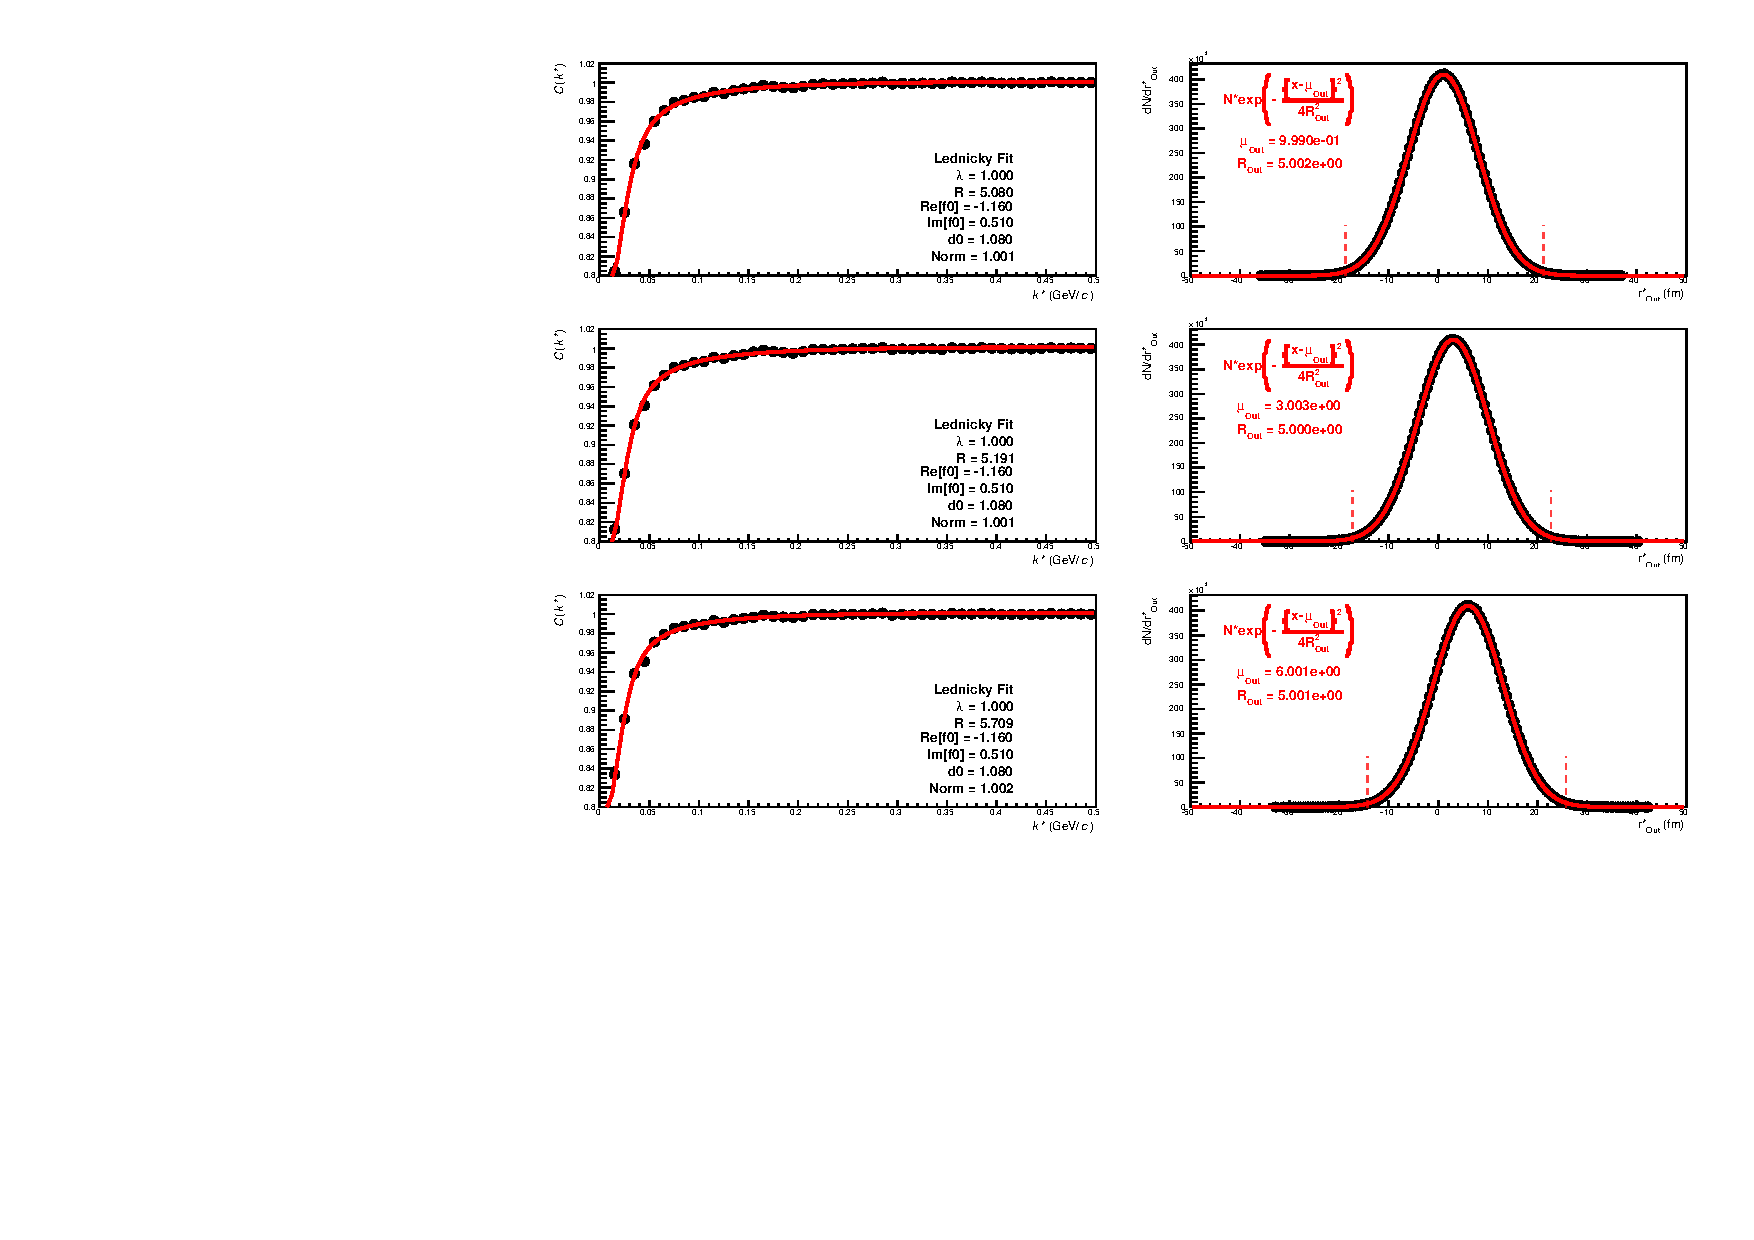
\includegraphics[width=\textwidth]{/home/jesse/Analysis/FemtoAnalysis/AnalysisNotes/7_ResultsAndDiscussion/7.1_ResultsLamK/7.1.5_ResultsLamK_DiscussionOfmTScaling/ThermPlots/LamKchP/CanCompMus_Full_LamKchP_3dHistPairSource3d_oslLamKchP.pdf}
  \caption[Short Caption]{Long Caption}
  \label{fig:LamKchP_ThermSources_VaryMuOut}
\end{figure}

















\clearpage
\end{document}